% document style header
\documentclass[a4paper, 12pt]{config/homework}

% import default packages
\usepackage{config/defpackages}
% import custom math commands
\usepackage{config/domath}
% for inserting pages
\usepackage{pdfpages}

% end preamble
\begin{document}

% document title
\noindent
\begin{tabularx}{\textwidth}{>{\centering\arraybackslash}X>{\centering\arraybackslash}X>{\centering\arraybackslash}X}
Calvin Sprouse & PHYS489 1B & 2024 Jan 19\\
\midrule
\end{tabularx}

% Select and write a reflection on a graded artifact (e.g., homework assignment, test, report) from one of the listed elective classes that you think best demonstrates the learning outcome of knowing key physical concepts and applying them to analyze and interpret the behavior of physical systems.
% The artifact you select should be from an elective upper division physics class, such as
% PHYS 301, 303, 304, 322, 323, 334, 410, 433, 441, 454, 475.
% (For students in the Biophysics Specialization, PHYS 322 and 323 are not considered electives.)

My chosen artifact for this goal is homework assignment 4 from PHYS322 Molecular Biophysics. This homework begins with some simple rate-based model questions regarding populations. My experience in differential equations was helpful in finding solutions to these two populations. I then looked at a MATLAB model of population dynamics considering a simple predator-prey system. This is another differential equation which can be solved for steady state solutions. I was able to find the interesting steady state solutions and demonstrate that small deviations from these solutions produce periodic oscillations in teh predator-prey populations. I really enjoyed working on question 5 of this assignment regarding the balance-point model. Figure 1 of question 5 shows experimental data and a linear fit that I developed for this assignment. The original data was not linear but simply taking the inverse of the length variable resulted in linear data. I preformed this linear fit using a Python notebook and the scipy package. Using the residuals I was able to compute an uncertainty in the linear fit and indicate that on the figure. This linear fit gave values which I then input to the simulation code and compared against experimental data. For the first comparison in Figure 2 I found poor fit in general but close shape agreement. I removed the first data point and in Figure 3 found much closer agreement to experimental data. This indicated to me that the first data point had some non-simulated characteristics. In the final figure I demonstrated that regardless of starting length the simulation predicts a convergence to a predicted balance-point length.

% artifact
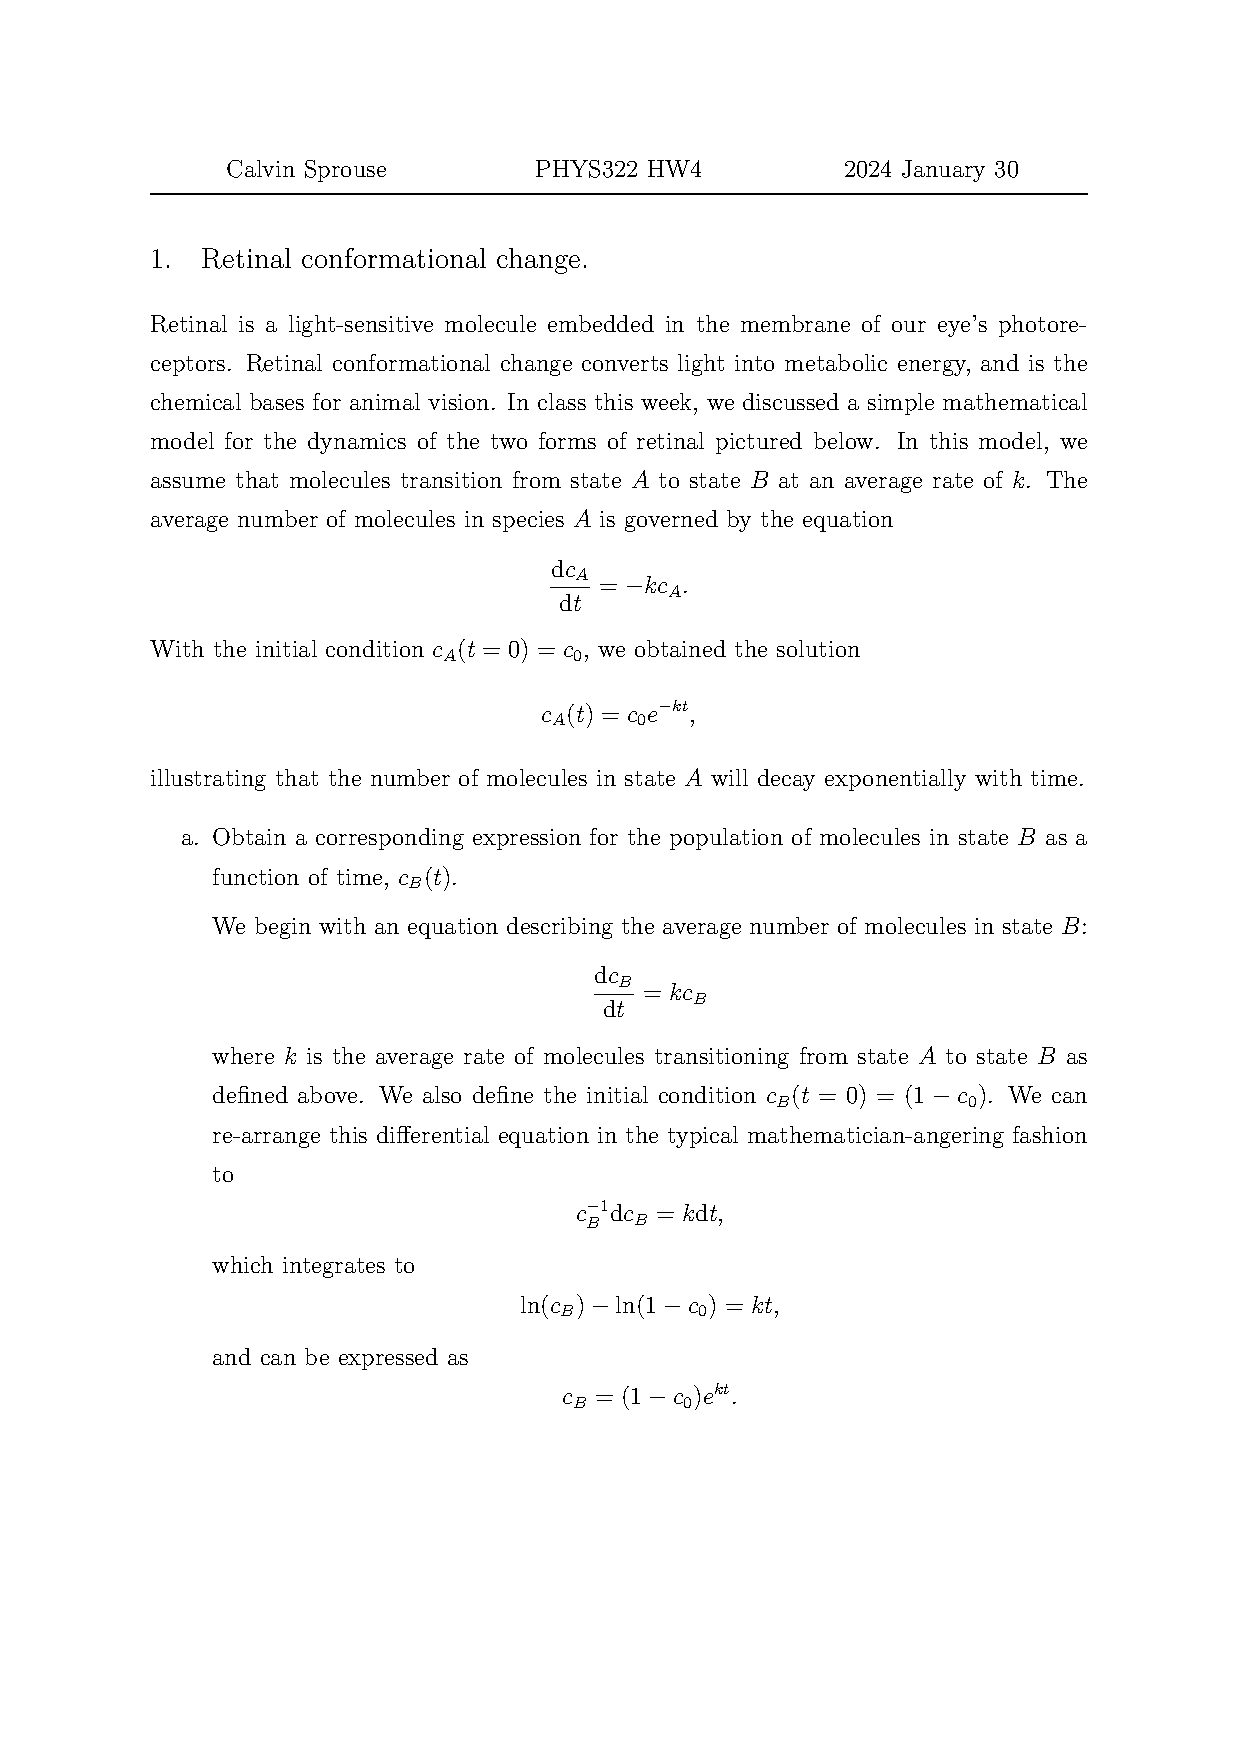
\includepdf[pages=-]{hw4.pdf}

\end{document}
